%%%%%%%%%%%%%%%%%%%%%%%%%%%%%%%%%%%%%%%%%%%%%%%%%%%%%%%%%%%%%%%%%%%
%                                                                 %
%                            CHAPTER FIVE                          %
%                                                                 %
%%%%%%%%%%%%%%%%%%%%%%%%%%%%%%%%%%%%%%%%%%%%%%%%%%%%%%%%%%%%%%%%%%%

\chapter{POPULATION COUNT AND OTHER STATISTICS} \label{sec:results}

%\begin{table*}[t]
\begin{table*}[!htb]%
    \centering
        \caption[Collected Image Totals by Species]{\textbf{Collected Image Totals by Species.}  The data collected during the GZGC was considered usable if it adhered to the collection protocol, meaning it was of sufficient quality and of the correct viewpoint.  Most of the unusable images were disregarded for being of an incorrect viewpoint.}
        \resizebox{\linewidth}{!}
    {
        \begin{tabular}{r|rrrrrrr}
                \hline
                \head{Species} & \head{Images} & \head{Usable Images} & \head{Citizen Scientists} & \head{Sightings} & \head{Usable Sightings} & \head{Identified} & \head{Estimated}\\
                \hline
                Plains Zebras & 5,550 & 3,609 & 55 & 8,659 & 4,545 & 1,258 & 2,307 $\pm$ 366 \\
                Masai Giraffes & 1,005 & 432 & 47 & 1,323 & 466 & 103 & 119 $\pm$ 48 \\
        \end{tabular}
    }
        \label{tab:collection}
\end{table*}

All of the results and metrics detailed in this chapter were generated and extracted using a prototype version of IBEIS on the data collected during the GZGC.  Alongside the study for plains zebra (\textit{Equus quagga}), the IBEIS team also administered a second, parallel study to count the number of Masai giraffes (\textit{Giraffa camelopardalis tippelskirchi}) in the Nairobi National Park.  The Masai giraffe study followed an identical procedure as described in the previous chapters except it replaced plains zebras with Masai giraffes.  The IBEIS computer vision algorithm was tuned for performance on each species independently.

\section{Population}

\begin{figure}[!htb]%
    \centering
    \subfloat {{ $\vcenter{\hbox{ 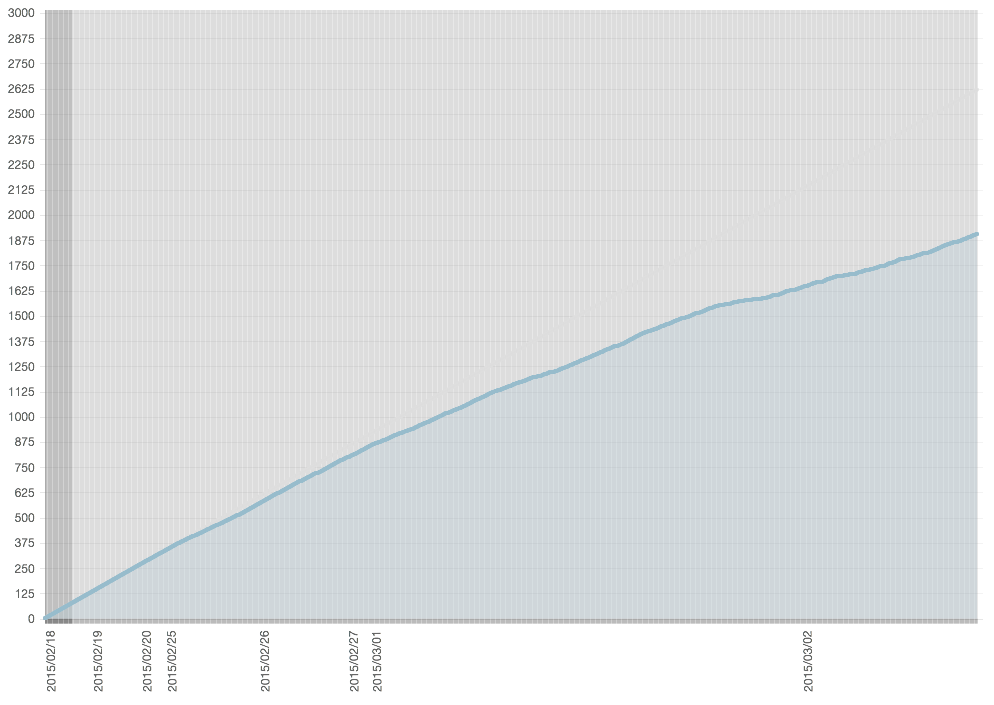
\includegraphics[width=0.45\textwidth]{resources/convergence_plains.png} }}$ }}%
    \subfloat {{ $\vcenter{\hbox{ 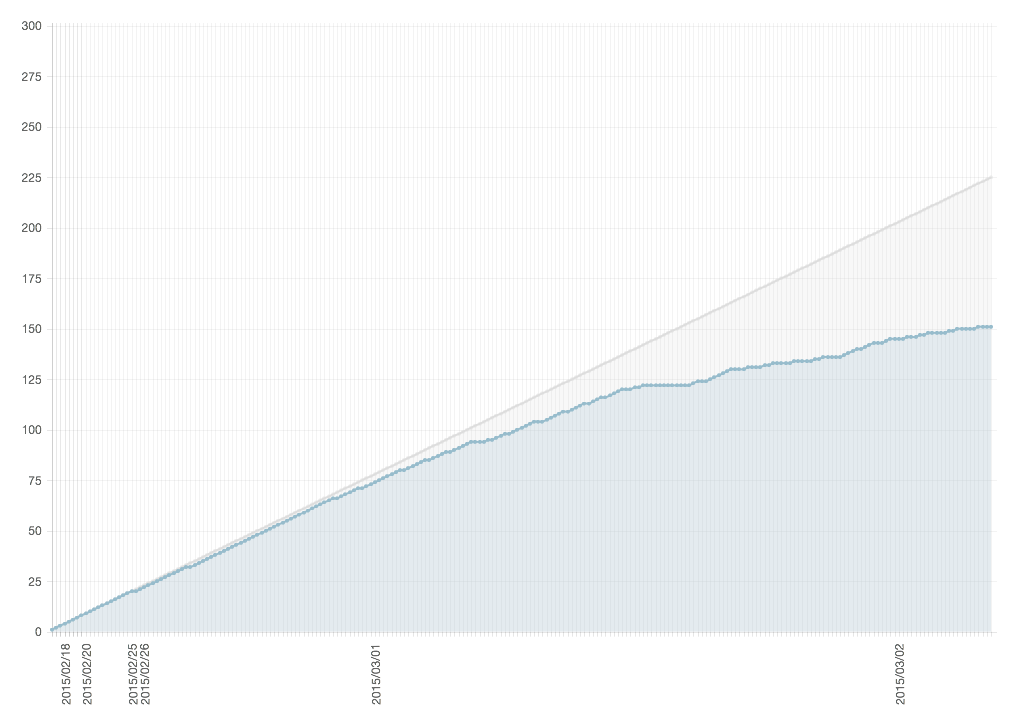
\includegraphics[width=0.45\textwidth]{resources/convergence_giraffes.png} }}$ }}%
        \caption[Rate of New Sightings by Images Taken of Zebra and Giraffe]{\textbf{Rate of New Sightings by Images Taken of Zebra and Giraffe.}  As images were taken of the zebra and giraffe populations, the probability of capturing a new individual decreased as the set of unseen animals became depleted.  The x-axis represents all chronological first sightings of a particular animal and the y-axis is the accumulation of total sightings over time.  The plot displays the rate of picture taking vs.\ the occurrence of a new animal.  The convergence of the identification is important to estimate the number of zebras (left) and giraffes (right).   The number of zebras is growing steadily as new images are processed, indicating that the actual plains zebra population has not been sufficiently sampled.  Conversely, the Masai giraffe population has begun to converge, which suggests that most of the giraffes in the park were sighted during the GZGC.  These trends coincide with the calculated Petersen-Lincoln indices from the mark-recapture study.}
        \label{fig:convergence}
\end{figure}

During the two events, 9,406 images were collected from 58 citizen scientists (including 7 IBEIS contributors that helped generate the initial identification database); 55 of those citizen scientists contributed images of plains zebras and 47 contributed images of Masai giraffes.  A total of 5,550 images contained plains zebras and a total of 1,005 images contained Masai giraffes.  However, not all of these images were unusable because some were of a wrong viewpoint or had poor quality.  After being filtered, a total of 3,609 valid images of plains zebras and 432 valid images of Masai giraffes were left.  Of the images collected for both species, a total of 8,659 sightings of plains zebra were detected by IBEIS (of which, 4,545 were valid) and a total of 1,323 sightings of Masai giraffes were found (of which, 466 were valid).  The 4,545 plains zebra sightings were identified by IBEIS to find a total of 1,258 unique individuals and the 466 sightings of Masai giraffe sightings were identified as 103 unique individuals.

During the GZGC, the IBEIS team performed a mark-recapture study \cite{krebs_ecological_1999, petersen_yearly_1896, pradel_utilization_1996, robson_sample_1964, seber_estimation_1982} where we calculated a Petersen-Lincoln index \cite{pacala_population_1985} for the plain zebra and Masai giraffe populations, as defined in Equation \ref{eq:index}.

\begin{equation}
    \label{eq:index}
    \begin{split}
        E_1 & = \text{sightings made on day 1} \\
        E_2 & = \text{sightings made on day 2} \\
        S & =  \text{sightings made on both day 1 and 2} \\
        \text{Index}_\text{Petersen-Lincoln} & = \ceil*{ \dfrac{E_1 * E_2}{S} } \\
        \text{Variance}_\text{Petersen-Lincoln} & = \ceil*{1.96 * \sqrt{\dfrac{E_1^2 * E_2 * (E_2 - S)}{S^3}} } \\
    \end{split}
\end{equation}

We calculated a Petersen-Lincoln index of 2,307 $\pm$ 366 (95\% accuracy) for plains zebras and an index of 119 $\pm$ 48 (95\% accuracy) for the Masai giraffe population.  The mark-recapture study suggests that 47.1\% to 64.8\% of the  plains zebras in the NNP have been uniquely identified by IBEIS and 61.7\% to 100.0\% of the Masai giraffes in the NNP have been uniquely identified, based on the total number of identified individuals from IBEIS and the estimated population count from the Petersen-Lincoln indices.  This information is summarized in Table \ref{tab:collection}.  The rate of new sightings over time as new images were processed by IBEIS can be seen in Figure \ref{fig:convergence}.  As we can see to the left, the rate of discovery for plains zebras is steadily rising and has not reached a stable asymptote.  The lack of convergence is validated by the mark-recapture study, which suggests that only around half of the zebras in the Nairobi National Park were sighted during the GZGC.  Conversely, the figure to the right shows the rate of new sighting for the Masai giraffes and does begin to flatten out, which suggests that the population of the giraffes in the NNP were adequately sampled during the GZGC.  The mark-recapture statistics for the giraffes suggest that there is a possibility that all of the giraffes in the park were identified.

The population estimate reported in this thesis does not come without some degree of sampling bias.  The two most severe forms of sampling bias with the GZGC were that the photographs originated from only locations where there were existing roads and that the images were only taken during daylight hours.  As such, any area of the NNP without a road was ignored during collection and no images were collected during night-time hours.  However, it is expected for a herd of zebras (even when only grazing) to move at least 1 kilometer within a 24 hour period \cite{juang_energy-efficient_2002, macedo_ecology_2010} and our sampling on multiple days increased the chances of capturing missed animals.  Moreover, the areas of the NNP that were not within a 1 kilometer distance of any road were limited.  Therefore, the property of equal catch-ability \cite{seber_estimation_1982, white_program_1999} largely applies here to \textit{where} an image was taken, but it also applies to \textit{when} it was taken.  The zebras on the Serengeti budget their time loosely independent of the daylighting conditions (i.e.\ they are continuously active and inactive during the day and night) \cite{becker_mother-infant_1990, kivai_feeding_2006, rubenstein_ecology_1994}, which lessens the severity of the time bias of when an image of an animal was captured.  Ultimately, these two biases could be directly addressed and overcome by using static camera traps that capture images at all hours of the day and either in areas with no roads or areas of significant congestion.  While we did not utilize them, future data collection events like the GZGC should consider using camera traps to help eliminate as much collection bias as possible.  The last form of bias that we wish to address is that of the individual personalities of the animals, which could have an effect on their (or their herd's) behavior: an individual is more shy or bold, is old or young, is more active or inactive, is pregnant, is nursing, is injured, etc.  These personality traits could have had an impact on the images collected during the GZGC.  However, we note that these personality traits would not have changed rapidly and would most likely have existed between the first and second days of the mark-recapture study.  As a result, we can mostly ignore these personality traits from biasing the accuracy of the population estimate.

\section{Demographics}

\begin{table}[!htb]
%       \begin{minipage}{.75\linewidth}
        \centering
            \caption[Plains Zebra and Masai Giraffe Age Distributions by Sex]{\textbf{Plains Zebra and Masai Giraffe Age Distributions by Sex.} A subset (262) of the identified plains zebra (top) and a subset (12) of the identified Masai giraffe (bottom) individuals could not be accurately aged or sexed (due to a limited number of images or viewpoints of that animal) and are thus ommitted from this table.}
        \scalebox{0.80}{
            \begin{tabular}{r|rrr|r}
                    \hline
                    \head{Sex} & \head{Infant} & \head{Juvenile} & \head{Adult} & \head{\textbf{Total}} \\
                    \head{} & \head{(0-12 mo.)} & \head{(12-36 mo.)} & \head{(36+ mo.)} & \head{} \\
                    \hline
                    Female (Zebra) & 46 & 83 & 342 & 471 \\
                    Male (Zebra) & 28 & 43 & 271 & 342 \\
                    \textit{Unknown} (Zebra) & 43 & 36 & 104 & 183 \\
                    \hline
                    \textbf{Total (Zebra)} & 117 & 162 & 717 &  996 \\
                    \hline
                    \hline
                    Female (Giraffe) & 3 & 9 & 35 & 47 \\
                    Male (Giraffe) & 0 & 10 & 31 & 41 \\
                    \textit{Unknown} (Giraffe) & 3 & 0 & 0 & 3 \\
                    \hline
                    \textbf{Total (Giraffe)} & 6 & 19 & 66 & 91 \\
            \end{tabular}
        }
            \label{tab:demographics}
%       \end{minipage}%
%   \hspace*{0.5 cm}
%       \begin{minipage}{.45\linewidth}
%       \centering
%       \scalebox{0.55}{
%           \begin{tabular}{r|rrr|r}
%                   \hline
%                   \head{Sex} & \head{Infant} & \head{Juvenile} & \head{Adult} & \head{\textbf{Total}} \\
%                   \head{} & \head{(0-12 mo.)} & \head{(12-36 mo.)} & \head{(36+ mo.)} & \head{} \\
%                   \hline
%                   Female & 3 & 9 & 35 & 47 \\
%                   Male & 0 & 10 & 31 & 41 \\
%                   \textit{Unknown} & 3 & 0 & 0 & 3 \\
%                   \hline
%                   \textbf{Total} & 6 & 19 & 66 & 91 \\
%           \end{tabular}
%       }
%           \caption[Masai Giraffe Age Distributions by Sex]{\textbf{Masai giraffe age distributions by sex.}  A subset (12) of the identified Masai giraffe individuals could not be accurately aged or sexed (due to a limited number of images or viewpoints of that animal) and are thus ommitted from this table.}
%           \label{tab:demographics-girm}
%   \end{minipage}
\end{table}

The demographics of the zebra and giraffe population can be compiled using the age and sex annotations provided by the trained biologists during the analysis.  Out of the total 1,258 identified zebra individuals, 996 of them had sufficient evidence to age and sex the animal (262 individuals had either poor sample images or poor viewpoints to confidently assign a sex or age).  As for the 103 identified individuals in the giraffe population, 91 of them had adequate images for them to be aged and sexed (12 individuals could not be confidently assigned age or sex).  The male to female ratio of the zebra population is 72.61\%, indicating a healthy breeding population \cite{hack_status_2002}.  The giraffes have a  87.23\% male to female ratio, which suggests a less stable population. %\cite{}
The full age and sex breakdown between plains zebras can be seen in Figure \ref{tab:demographics} (top) and (bottom) for Masai giraffes.  When we look at these population estimates based on our photographic censusing, it is clear to see the advantages over the currently used counting methods \cite{ogutu_changing_2013}.  Our method simplifies image collection by utilizing citizen scientists (freeing up administrative man power) and provides more detailed population estimates with tighter confidence bounds.

Using Pearson's chi-squared \cite{plackett_karl_1983, rao_analysis_1981} contingency table analysis, the age demographics of the NNP zebra population can be compared to the demographics of other stable populations, such as the general zebra population on the Serengeti.  Based on previous studies \cite{fitzgibbon_antipredator_1995, macedo_ecology_2010, sinclair_density_1996}, stable populations tend to have at least 25\% recruits (infants and juveniles).  Table \label{tab:demographics-pz} shows that 28\% of the Nairobi National Park zebra population consists of recruits, which suggests that zebra population on the NNP is also stable. This contrasts with the age demographics of plains zebras on the Borana and Ol Pejeta conservancies in central Kenya where lion densities are very high and recruits only comprise around 12\% \cite{macedo_ecology_2010}.  For giraffes, recruits comprise 27.5\% of the population, but we cannot determine if the population is stable due to the lack of a suitable comparison study performed on the Serengeti.

The demographics of the zebra and giraffe populations give the wildlife managers at the NNP the reproductive data to help maintain a healthy population or to limit overpopulation by selectively removing animals from breeding, transferring animals to another park, or by introducing more natural predators.  The age information generated can ultimately be used, if a study similar to the GZGC is continued over several years, to predict the average life-expectancy for the population.  The life-expectancy can be compared to previous years or be used as a comparison for the overall health of the population compared to other conservancies.

\section{Concentration and Movement}

\begin{figure}[!htb]%
    \centering
    \subfloat {{ $\vcenter{\hbox{ 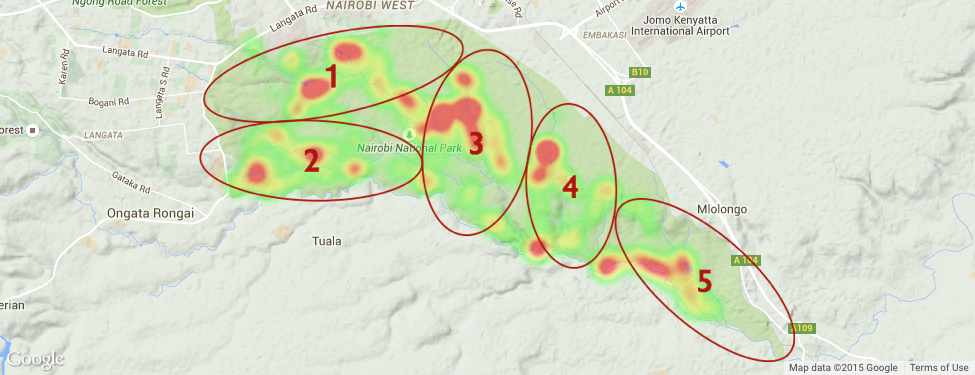
\includegraphics[width=0.90\textwidth]{resources/coverage2.png} }}$ }}%
        \caption[Concentration and Sampling Locations in the Nairobi National Park]{\textbf{Concentration and Sampling Locations in the Nairobi National Park.}  The concentration map of sightings taken during \textit{The Great Zebra \& Giraffe Count} show missing regions of the park that were under-sampled (north-east boundary) and need to be explicitly covered in future population surveys.  The concentration map shows that all assigned (5) zones during the GZGC were samped during collection.  The color red indicates that 150 (or more) images were taken at that location; the color gradient decreases linearly where yellow indicates 100 images and green indicates 50 images.}
        \label{fig:coverage}
\end{figure}

Using the corrected GPS data, a model of where the animals were sighted throughout the park can be generated.  Note that the estimation for the concentration of the animals is heavily biased to the locations and tracks of the vehicle-permissible roads in the NNP.  As a result, some parts of the park were under-sampled or completely missed during the GZGC.  However, performing the data collection event over many days increases the likelihood of capturing images of animals due to their natural migration and grazing movement.  A concentration map, seen in Figure \ref{fig:coverage}, can be used by the conservationists to identify areas of the park that are being over-grazed, are not being actively monitored, or are simply unpopular to certain species due to natural predators, environmental conditions (e.g.\ water and grazing resources, natural cover, or safety), or human interaction.  The locations of the park that the animals shy away from can be artificially enhanced using incentives such as water, nutrients, or shelter.  Locations with minimal animal traffic can also be earmarked for future infrastructure development as any new structures would ideally like to have minimal impact on the ecosystem and the behavior of the animals.

It is important to note that any analysis on the concentration and movement will seem sporadic at any given time.  As a result, the monitoring of the population using GPS should be done continuously to generate a more representative picture of the population's movements.  Having data over time allows the park to predict the movement of the animals based on weather conditions, seasons, or natural migration and can be used to help plan better infrastructure and focus maintenance efforts on heavily traversed areas.
